\clearpage\begingroup\SourceLeaf{29b}\HistoricalHead{24}{L}{PHYSIK. BRIEFWECHSEL.}
\begin{center}
[3.]\\[.7em]
\textsc{Gauss} an \textsc{Schumacher}. Göttingen, 23. April 1836.
\par\medskip\rule{.78\textwidth}{.35pt}\par
{\small [Briefwechsel zwischen \textsc{Gauss} und \textsc{Schumacher}, III, Altona 1860, S. 51.]}\par
\rule{.78\textwidth}{.35pt}
\end{center}
\noindent .\ .\ .\ .\ .\ .\ .\ .\ .\ .\ .\ .\ .\ .\ .\ .\ .\ .\ .\ .\ .
\par\noindent\hspace*{\parindent}Da Sie selbst an Ihrer Waage keine Libelle angebracht haben (auch
nach Ihren Mittheilungen in der That keiner bedürfen), so ist Ihnen vielleicht
nicht uninteressant, wenn ich auf einen, wie mir deucht, wesentlichen Umstand,
in Beziehung auf Verbindung der Libelle mit der Waage, aufmerksam
\clearpage\SourceLeaf{30}\HistoricalHead{25}{R}{GAUSS AN SCHUMACHER.}
\noindent mache. Sollten Sie denselben schon früher in Erwägung genommen haben,
so bitte ich das folgende zu überschlagen und zu entschuldigen.

Findet eine solche Verbindung Statt, und entspricht also einer auch nur
äusserst wenig veränderten Neigung des Waagbalkens eine \textls[120]{vergleichungsweise}
beträchtliche Verrückung der Blase, so entsteht dadurch eine \textls[120]{erhebliche
Veränderung des Moments}; die Waage bekommt dadurch also
selbst eine vergrösserte Empfindlichkeit, die leicht so sehr vergrössert werden
kann, dass sie ganz umschlägt, oder gar kein stabiles Gleichgewicht mehr
möglich ist. Natürlich werden Sie mir nicht entgegensetzen, dass bei dem
so geringen Gewicht der Luftblase eine Veränderung ihres Moments ganz
unmerklich sein müsse; denn genau betrachtet ist es nicht das Moment des
Luftkörpers, sondern eines gleich grossen Spiritusvolumens, von dem hier die
Rede ist.

\noindent\begin{minipage}[t]{.69\textwidth}\setlength{\parindent}{1.2em}\indent
Wenn nemlich die Blase von \(A\) nach \(B\) fortgerückt
ist, so ist nicht das Product \(AB\times\) Gewicht der Luft
in der Blase das worauf es ankommt, sondern dieses
\end{minipage}\hfill
\begin{minipage}[t]{.28\textwidth}\vspace{-1.4ex}\centering
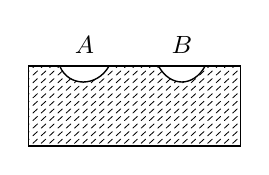
\begin{tikzpicture}[x=.0048cm,y=-.0048cm,line width=.5pt,line cap=round]
\begin{scope}
\clip (32,72)--(115,72)..controls (138,128) and (214,128)..(245,72)--(376,72)..controls (407,128) and (468,128)..(499,72)--(592,72)--(592,283)--(32,283)--cycle;
\foreach \y in {76,96,...,296}{\foreach \x in {22,44,...,616}{\draw[line width=.3pt] (\x,\y)--++(12,-11);}}
\end{scope}
\draw (32,72) rectangle (592,283);
\draw (115,72)..controls (138,128) and (214,128)..(245,72);
\draw (376,72)..controls (407,128) and (468,128)..(499,72);
\node[anchor=south,font=\small] at (180,66) {\(A\)};
\node[anchor=south,font=\small] at (438,66) {\(B\)};
\end{tikzpicture}
\end{minipage}\par\noindent
Gewicht mag man ganz ignoriren und nur bedenken, dass durch jene Veränderung
so viel Spiritus als vorher in \(B\) war, nach \(A\) gekommen ist. Eine solche
Momentsveränderung ist aber wie gesagt vergleichungsweise etwas sehr beträchtliches.
Es wird dadurch ceteris paribus um so leichter das Umschlagen
(also völlige Unbrauchbarkeit der Waage in diesem Zustande) erfolgen,
\par\noindent\hspace*{\parindent}1) je empfindlicher die Waage ohne Libelle für sich war,
\par\noindent\hspace*{\parindent}2) je kleiner ihre Belastung,
\par\noindent\hspace*{\parindent}3) je empfindlicher (kleinkrümmiger) die Libelle,
\par\noindent\hspace*{\parindent}4) je grösser die Blase.
\par\noindent\hspace*{\parindent}Es folgt hieraus, dass jenes Mittel zwar bei Waagen für grosse Belastung
(z. B. à 50 {\fontspec{FreeSerif.otf}℔}) herrliche Dienste thun kann. Soll aber eine Libelle bei einer
Waage für geringe Belastungen angewandt werden, so darf jene nicht sehr
empfindlich sein, muss eine kleine Blase haben, und die übrige Einrichtung
der Waage muss so sein, dass sie vor Anbringung der Libelle nur sehr geringe
Empfindlichkeit hat. Bei meiner eignen Waage, obgleich gerade ihre
Empfindlichkeit zu klein ist, bringt[\textsuperscript{*})]\begingroup\renewcommand{\thefootnote}{}\footnotetext{[\textsuperscript{*}) Die Handschrift hat \textls[120]{bewirkt}.]}\endgroup\ doch das Anbringen der kleinsten und
\HistoricalFoot{XI{\scriptsize 1}.}{4}
\clearpage\SourceLeaf{31}\HistoricalHead{26}{L}{PHYSIK. BRIEFWECHSEL.}
\noindent am wenigsten empfindlichen Libellenröhre, über die ich disponiren kann, und
trotz der sehr kleinen Blase, noch selbst bei Belastung mit 500 Grammen in
jeder Schale die Waage zum Ueberschlagen. (Ich hatte die Libelle unter
dem Waagbalken angebracht; \textls[120]{darüber}, ist natürlich das Umschlagen noch
\textls[120]{leichter}.) Da nun ohnehin die Blase durch Temperaturveränderung im Lauf
des Geschäfts sich ändern kann, und jede Aenderung der Blase auch den
Ausschlagswerth ändern muss, so ist mir noch zweifelhaft, ob bei Waagen
für mässige Belastung das Anbringen einer Libelle überhaupt zu rathen ist.
Jedenfalls würde es sehr schwierig sein, die Einrichtung so zu treffen, dass
man die Waage à deux mains, heute mit, morgen ohne Libelle brauchen
könnte.\quad .\ .\ .\ .\ .\ .\ .\ .\ .\ .\ .\ .\ .\ .\ .\ .\ .\ .\ .\ .\ .\ .\ .\ .
\clearpage\endgroup
